
\begin{frame}[fragile]{Construction d'un moteur de recherche}
  \begin{itemize}
    \item On va utiliser la base des films de MongoDB et l'indexer
    \item Dans Solr, un index s'appelle {\bf core}
    \item Celui par défaut que l'on a utilisé s'appelait ``collection1''
    \item On va en configurer un autre, ``movies''
  \end{itemize}
  \begin{itemize}
    \item Dans solr/example/solr :\\
\begin{minted}[frame=lines,
               baselinestretch=.9,
               fontsize=\footnotesize,
               framesep=2mm]{bash}
   cp -R  collection1 movies
   cd movies
\end{minted}
\item éditer ``core.properties'' pour changer 
la propriété \texttt{name} à \texttt{movies}
\item vider data/ :\\
  \begin{minted}[frame=lines,                                                     
               baselinestretch=.9,                                              
               fontsize=\footnotesize,                                          
               framesep=2mm]{bash}                                              
rm -Rf data/*
\end{minted} 
     \item se placer dans le répertoire ``conf''
  \end{itemize}
\end{frame}
       

%Pour indexer notre base nous allons donner à Solr des *documents Solr* que vous pouvez récupérer
%à partir du Webscope. La seule différence avec la représentation JSON complète est que
%les artistes sont représentés simplement par leur nom et prénom. Voici un exemple,
%qui nous donne donc les champs à indexer.

%.. code-block:: javascript
\begin{frame}[fragile]{Un document (exemple)}
  \begin{minted}[frame=lines,                                                     
               baselinestretch=.9,                                              
               fontsize=\footnotesize,                                          
               framesep=2mm]{json}
{
  "_id": "movie:57",
  "title": "Jackie Brown",
  "year": "1997",
  "genre": "crime",
  "summary": "Jacky Brown, hotesse de l'air, ...",
  "country": "USA",
  "director": "Quentin Tarantino",
  "actors": ["Robert De Niro", "Pam Grier", "Bridget Fonda",
                 "Michael Keaton","Samuel Jackson"]
}
\end{minted} 
\end{frame}

\begin{frame}{Schéma de l'index }
  \begin{itemize}
    \item Le schéma donne la liste de tous les champs d'un doc Solr
    \item Nombreuses options : 
      \begin{itemize}
        \item type (numérique, entier)
        \item possibilité de calcul de la valeur du champ à partir d'un autre
        \item traitements divers sur les valeurs du champ
      \end{itemize}
  \end{itemize}
\end{frame} % ending frame Schéma de l'index 

\begin{frame}[fragile]{Squelette}
  \begin{minted}[frame=lines,                                                     
               baselinestretch=.9,                                              
               fontsize=\tiny,                                          
               framesep=2mm]{xml}
   <?xml version="1.0" encoding="UTF-8" ?>

   <schema name="example" version="1.5">
    <!--  Liste des champs de l'index -->
  <fields>
    <field name="_id" type="string" indexed="true" stored="true" required="true" />
    <field name="title" type="string" indexed="true" stored="true" required="true" />
    <field name="summary" type="text" indexed="true" stored="false" required="false" />
    <!-- A completer -->

    <!-- Un champ dans lequel on concatene les autres pour une recherche "plein-texte" -->
    <field name="text" type="text" indexed="true" stored="false"
      multiValued="true" />
    <copyField source="summary" dest="text" />
    <copyField source="title" dest="text" />

        <!-- Un champ "technique" requis par Solr/Lucene -->
    <field name="_version_" type="long" indexed="true" stored="true" />
  </fields>

  <!-- La cle d'acces a un document dans l'index -->
  <uniqueKey>_id</uniqueKey>

    <!-- Configuration des types de champ -->
  <types>
    <fieldType name="string" class="solr.StrField" />
    <fieldType name="int" class="solr.IntField" />
    <fieldType name="long" class="solr.LongField" />
    <fieldType name="text" class="solr.TextField">
      <analyzer>
        <tokenizer class="solr.StandardTokenizerFactory" />
                <filter class="solr.LowerCaseFilterFactory" />
      </analyzer>
    </fieldType>
  </types>
   </schema>
  \end{minted}
\end{frame}

\begin{frame}{Squelette de l'index}
%Il comprend trois parties:

  \begin{itemize}
    \item la liste des champs, dans l'élement ``fields``, complétée par l'indication du champ de recherche par défaut;
    \item le champ qui identifie le document Solr, dans l'élément ``uniqueKey``;
    \item la liste des {\bf types de champ}, dans l'élément ``types``.
  \end{itemize}
  \bigskip
  Note : Pour des besoins internes, tout schéma doit contenir un champ ``\_version\_`` défini comme ci-dessus.
\end{frame} % ending frame Squelette de l'index

  
\begin{frame}{Définition des types et de la clé}
  \begin{itemize}
    \item Chaque type utilisé dans le schéma d'un index doit apparaître dans un
      des élements \variable{fieldType} du fichier {\bf schema.xml}
    \item Solr fournit tout un ensemble de types pré-définis qui suffisent pour      
      les besoins courants;  on peut associer des options à un type
%    \item Pour simplifier, disons qu'un type Solr correspond à une classe Java
%      (du nom du type)

        \item Les options indiquent d'éventuels traitements à appliquer                       
          à chaque valeur du type avant son insertion dans l'index
        \item ex: type \variable{text}
      \begin{itemize}
        \item on lui définit un ``analyseur''  ``StandardTokenizerFactory''
        \item se charge de découper le texte en {\bf tokens} pour une recherche
          plein-texte (détails plus tard)
        \item retenir : cela permet d'indexer chacun des mots, et donc de faire
          des recherches sur toutes les combinaisons de mots
      \end{itemize}
    \item  L'élément  \variable{uniqueKey} permet de rechercher un document dans
      l'index par sa clé. Indispensable, ne serait-ce que pour savoir qu'un
      document est indexé\\
 %     (le définir systématiquement semble une bonne pratique)
  \end{itemize}

\end{frame}

\begin{frame}[fragile]{Définition des champs}
\begin{minted}[frame=lines,
               baselinestretch=.9,
               fontsize=\footnotesize,
               framesep=2mm]{xml}
  <field name="_id" type="string" indexed="true" stored="true" 
        required="true" multiValued="false" />
\end{minted}
\smallskip
\begin{itemize}
  \item Les attributs de l'élement XML caractérisent le champ
  \item  Le {\bf nom} et le {\bf type} sont les informations de base
  \item Ensuite, divers attributs (souvent optionnels) :
    \begin{itemize}
      \item \variable{indexed} indique simplement que le champ pet être utilisé dans une recherche;  
      \item \variable{stored} indique que la {\bf valeur} du champ est {\bf stockée} dans l'index,
            et qu'il est donc possible de récupérer cette valeur comme résultat
            d'une recherche, {\bf sans avoir besoin de retourner à la base principale};
            en d'autres termes, ``stored`` permet de traiter l'index {\bf aussi} comme une
            base de données;
      \item \variable{required} indique que le champ est obligatoire;
      \item enfin, \variable{multivalued} vaut \variable{true} pour les champs ayant plusieurs
    valeurs, soit, concrètement, un {\bf tableau} en JSON; c'est le
    cas par exemple pour le nom des acteurs.
    \end{itemize}
    \end{itemize}
\end{frame}
\begin{frame}[fragile]{Définition des champs}
 Les champs \variable{indexed}  et \variable{stored} sont très
        importants
\vfill
Toutes les combinaisons de valeur sont possibles :
    \begin{itemize}
      \item \variable{indexed=true}, \variable{stored=false}: on pourra interroger
      le champ, mais il faudra accéder au document principal dans la  base documentaire si on veut sa valeur;
    \item \variable{indexed=true}, \variable{stored=true}: on pourra interroger
      le champ, {\bf et} accéder à sa valeur dans l'index;
    \item \variable{indexed=false}, \variable{stored=true}: on ne peut pas interroger le champ, mais
      on peut récupérer sa valeur dans l'index;
    \item \variable{indexed=false}, \variable{stored=false}: n'a pas de sens à priori; le seul intérêt
      est d'ignorer le champ s'il est fourni dans le document Solr.
    \end{itemize}

\end{frame}

\begin{frame}[fragile]{Définition des champs (suite)}
Comment peut-on indexer un champ sans le stocker ?
  \begin{itemize}
    \item c'est notamment le cas pour les textes qui sont décomposés en
      {\bf termes}: chaque terme est indexé indépendamment
    \item très difficile pour l'index de reconstituer le texte
    \item d'où l'intérêt de conserver ce dernier dans son  intégralité, à part
  \end{itemize}

\vfill

C'est une question de compromis: 
\begin{itemize}
  \item {\bf stocker} une valeur prend plus d'espace que {\bf l'indexer}
  \item Dans la situation la plus extrême, on dupliquerait la base documentaire
    en stockant chaque document {\bf aussi} dans l'index
  \item un stockage plus important dégrade les performances
\end{itemize}
\begin{comment}
\bigskip
Y a-t-il une valeur par défaut pour ces options ?
\begin{itemize}
  \item les valeurs par défaut de  \variable{indexed} et \variable{stored} 
   par exemple sont {\bf héritées} du type du champ (par exemple \variable{TextField}), 
 \item pour le type,  on ne sait pas toujours comment c'est défini.
 \item il est donc {\bf préférable de toujours les mettre explicitement}
\end{itemize}
\end{comment}
\end{frame}

\begin{frame}{}
 
\vfill
 
 Le squelette de schéma comprend également un champ {\em calculé}, le champ
      \variable{text}. 
      
\vfill
      
 Les instructions \variable{copyField} indiquent qu'au moment de l'insertion d'un document,
on va ``copier'' certains champs dans celui-ci. 

\vfill

  \begin{itemize}
    \item le type du champ  \variable{destination} correspond à un mode particulier d'indexation, éventuellement
      différent et complémentaire de celui du champ \variable{origine}; 
      
      => par exemple le contenu d'un titre
    est indexé comme une chaîne de caractères dans le champ \variable{title}, et comme un texte
    "tokenisé" quand on le copie dans le champ \variable{text};
  \item si {\bf toutes} les occurrences de chaînes de caractères sont concaténées
   dans un même champ,
    on obtient, en prenant ce champ pour cible, une recherche plein-texte globale. 
  \end{itemize}

\end{frame}


 \begin{frame}{Recharger le schéma}
   \begin{itemize}
     \item Après tout changement de schéma, il faut {\bf recharger} l'index. 
     \item Pour recharger un index, à partir de l'interface d'administration, utilisez l'option
{\bf Reload} après avoir sélectionné le {\bf core}
   \end{itemize}
   \begin{center}
     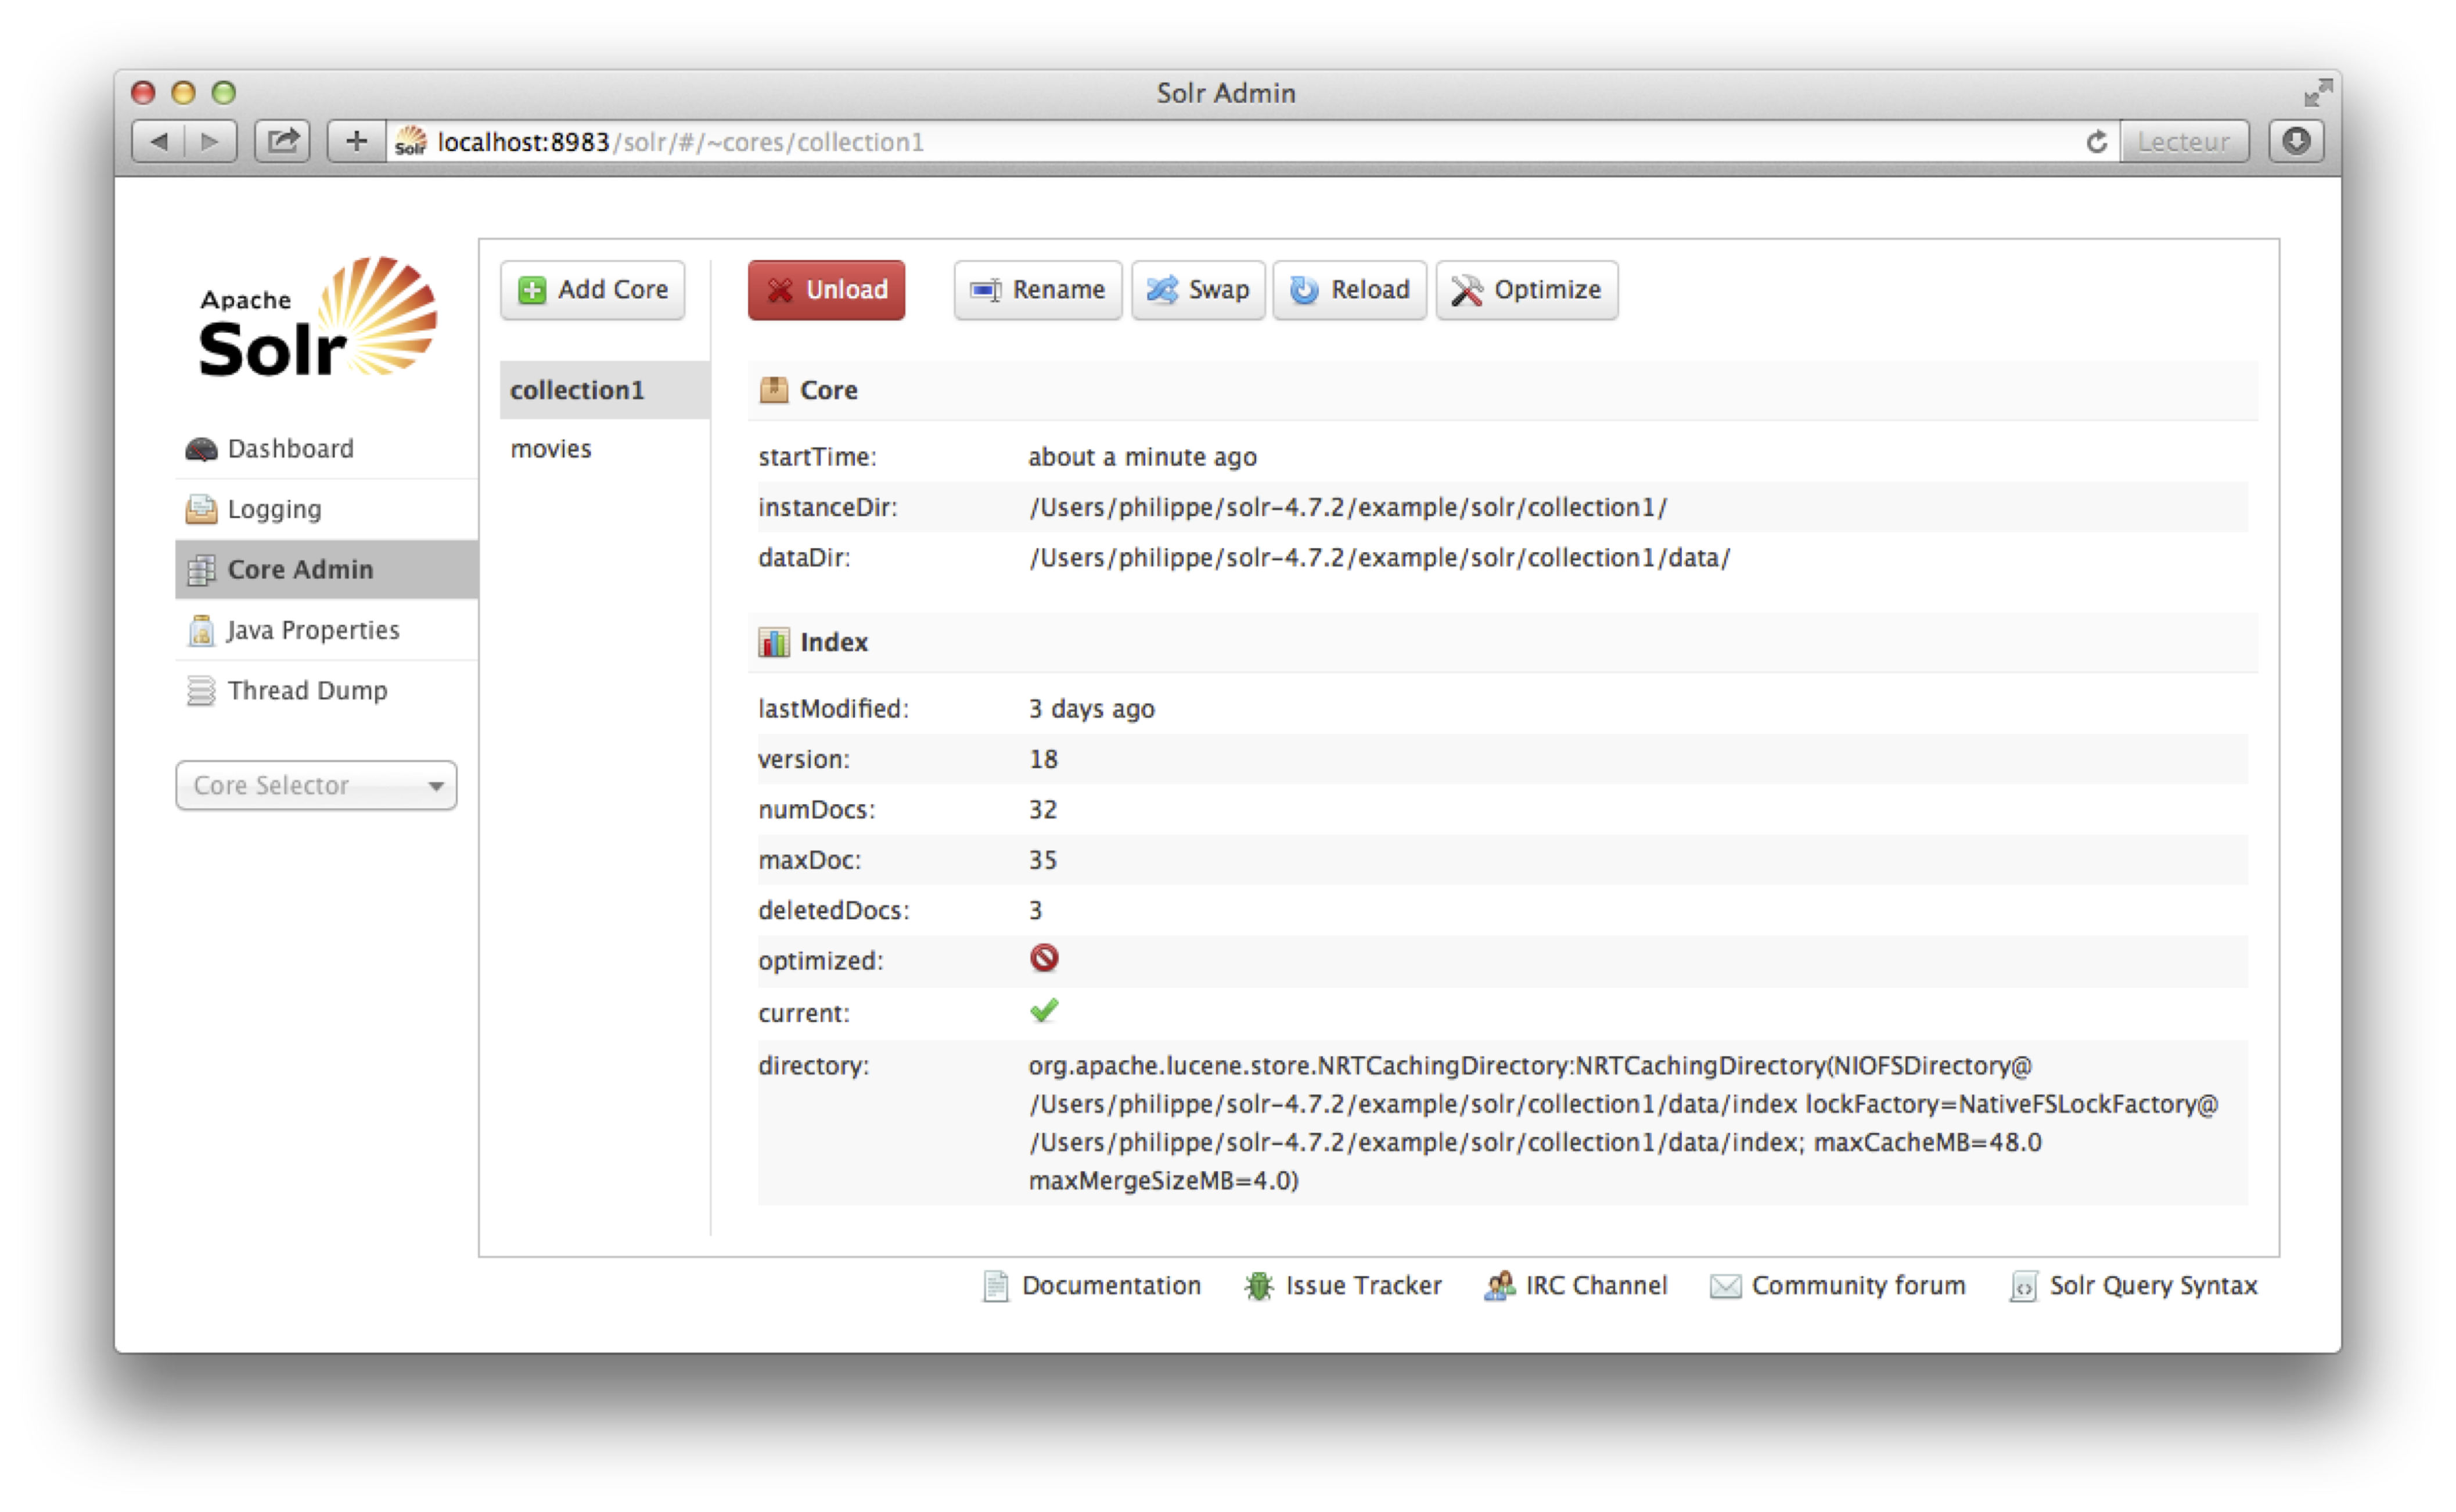
\includegraphics[height=6cm]{../figures/solr-reload.png}
   \end{center}
 \end{frame}

\begin{frame}[fragile]{Rechargement}

\begin{minted}[frame=lines,
               baselinestretch=.9,
               fontsize=\footnotesize,
               framesep=2mm]{bash}
    curl "http://localhost:8983/solr/movies/update/json?commit=true" \\
    --data-binary @solr_doc.json -H "Content-type:application/json"
\end{minted}

\begin{itemize}
  \item Attention, si l'index existant ne correspond pas au nouveau schéma, le rechargement échouera. 
  \item Avec Solr, il est (plus) difficile de faire évoluer un schéma (qu'avec BDD classique)
\end{itemize}
\smallskip
Reconstruction (destruction puis validation) :
\begin{minted}[frame=lines,
               baselinestretch=.9,
               fontsize=\footnotesize,
               framesep=2mm]{bash}
    curl http://localhost:8983/solr/movies/update  \\
        --data "<delete><query>*:*</query></delete>" \\
        -H "Content-type:text/xml; charset=utf-8"
    curl http://localhost:8983/solr/movies/update \\
      --data "<commit/>' -H 'Content-type:text/xml; charset=utf-8"
\end{minted}
\end{frame}

